
\chapter{Methodology}
\label{ch:methodology}

In this chapter, we describe the methodological approach for the literature search, describe the system used behind the literature search and give an idea on the scale of this topic. Furthermore, we are going to introduce the methodology for the empirical evaluation.

% \subsection{Research Questions} \label{appendix:method:rq}
% not adapted...
% Research questions aim to provide a structure and help the reader to follow. We defined the following research questions which will lead through the paper:
% \begin{enumerate}
%     \item What are the key characteristics of proposed watermarking and fingerprinting methods?
%     \item Can the watermarking method be extended to fingerprinting?
%     \item How are the different methods comparable?
%     \item What are the methods vulnerable to?
%     \item Do other IP protection methods exist besides of watermarking and fingerprinting?
% \end{enumerate}

\section{Literature search} \label{appendix:method:search}

\begin{figure} %h!
 \centering
 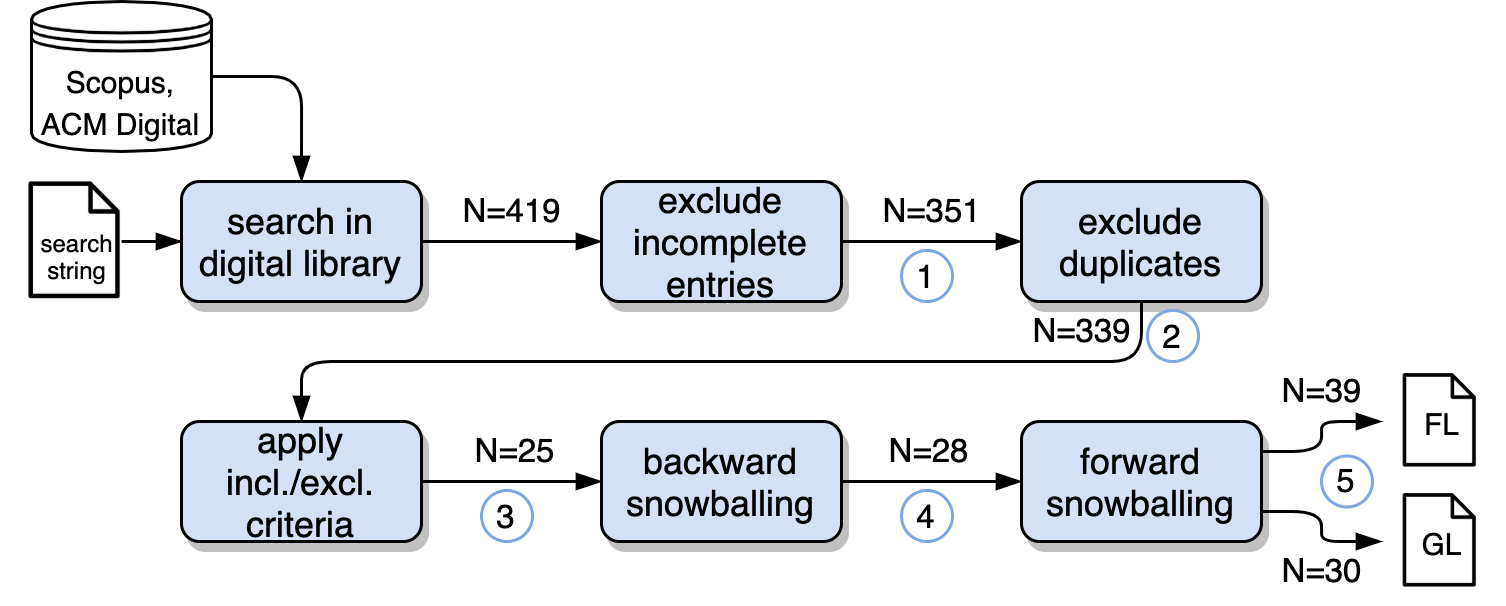
\includegraphics[width = 0.7\textwidth]{images/search-process.png}
 \caption{Literature search process workflow. In every step we denote the number of publications by $N=x$. The numbers 1 to 6 correspond to the CSV-files which contain all the retrieved literature in the particular step.}
 \label{fig:search-process}
\end{figure}

In preparation for this master thesis, we performed an extensive literature search and documented every step to make it reproducible. \cref{fig:search-process} shows the workflow of our literature search process. The complete documentation of the search process including the search strings and results with the retrieved literature will be made available in the GitHub project \url{https://github.com/mathebell/model-watermarking}.

We distinguish between the following types of publications: \textit{formal literature} (FL), i.e. peer-reviewed literature such as book sections, conference papers, journal articles, and \textit{grey literature} (GL), i.e. literature that did not undergo a peer-review process, such as pre-prints (published on repositories such as arXiv, or university repositories, author's websites, etc.) However, in its definition, grey literature does not only consist of pre-prints but can also be formed by blogs, interviews, wikis and many more document types \cite{mahood_searching_2014}, \cite{noauthor_greynet_nodate}. In this thesis, as the subject of watermarking of ML models has not produced such types of GL yet, it does however only consist of pre-prints.

\begin{figure} 
 \centering
 \begin{subfigure}[b]{0.48\linewidth}
 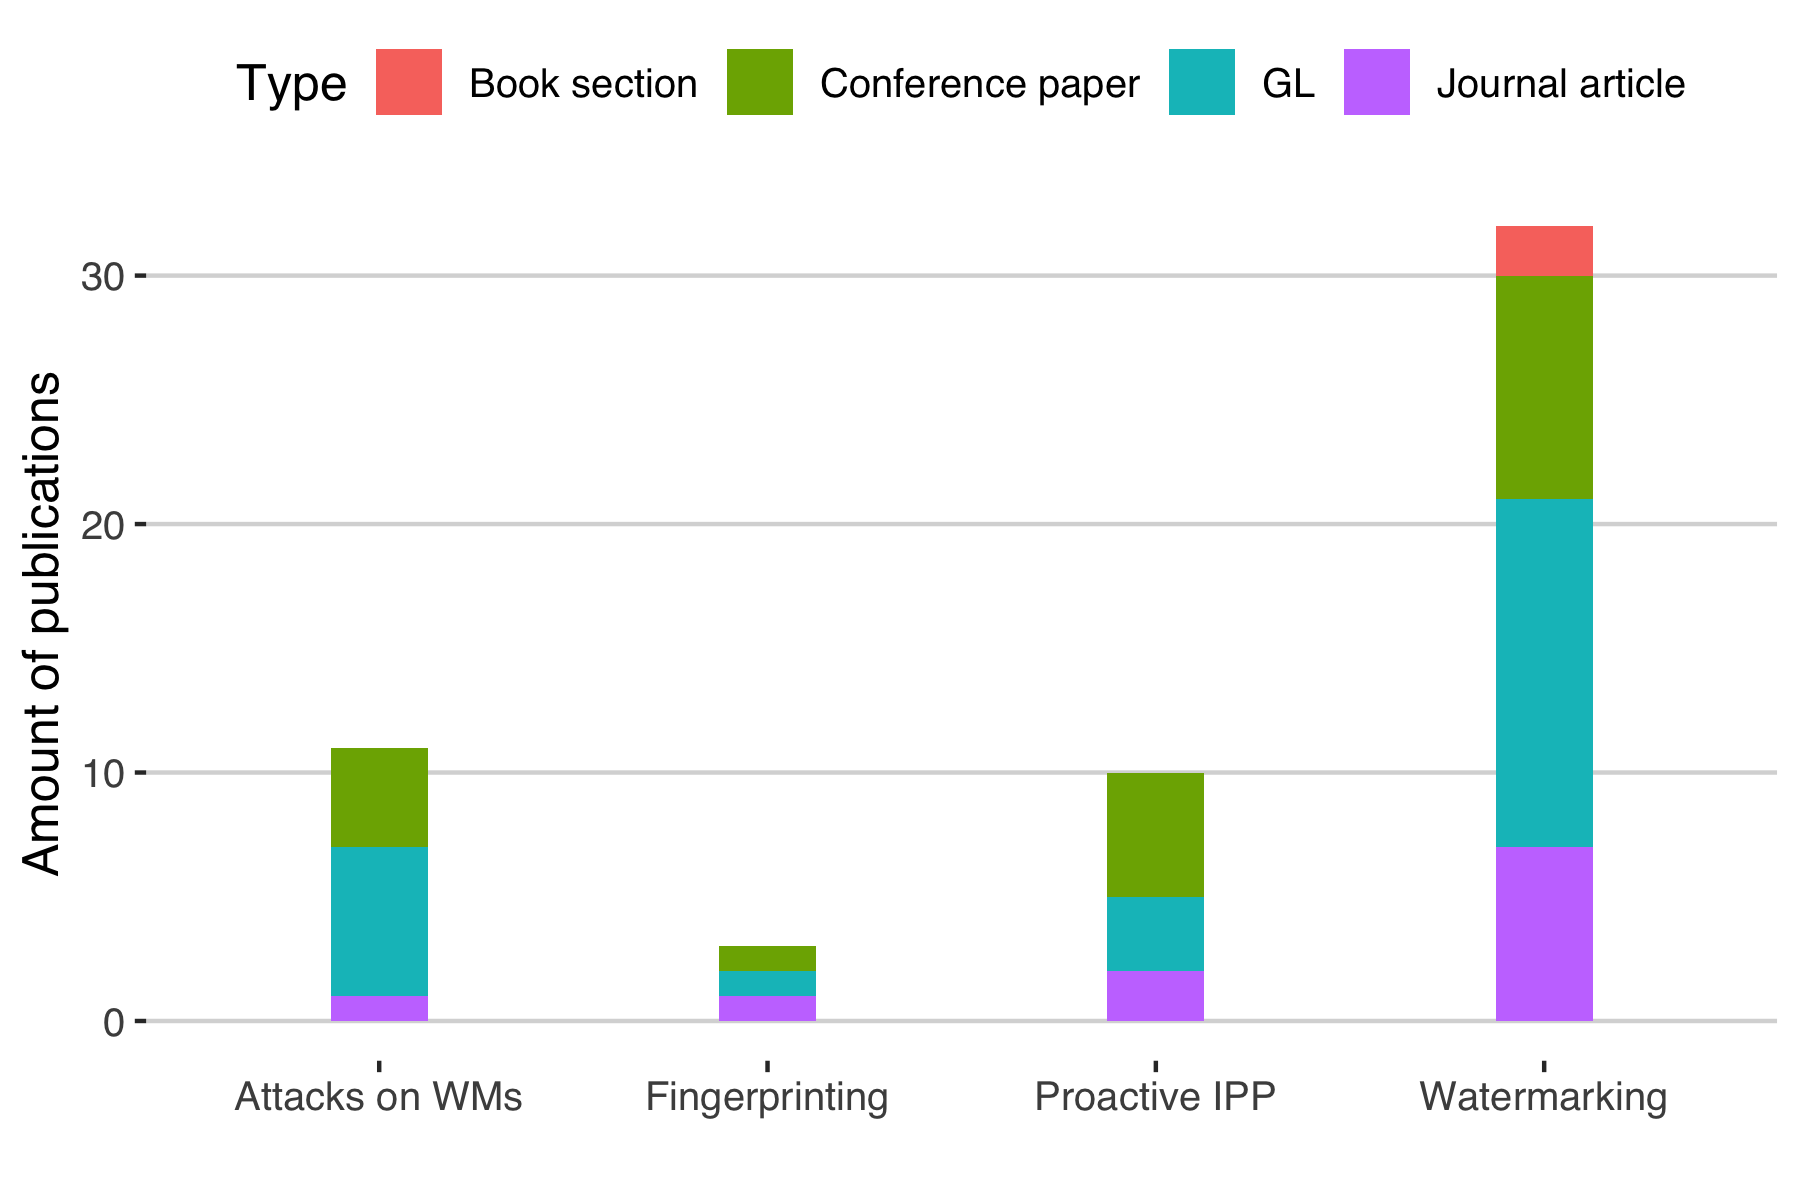
\includegraphics[width =\linewidth]{images/literature_types.png}
 \caption{Across different topics regarding ML IPP}
 \label{fig:aufteilung}
 \end{subfigure}
 \hfill
 \begin{subfigure}[b]{0.48\linewidth}
 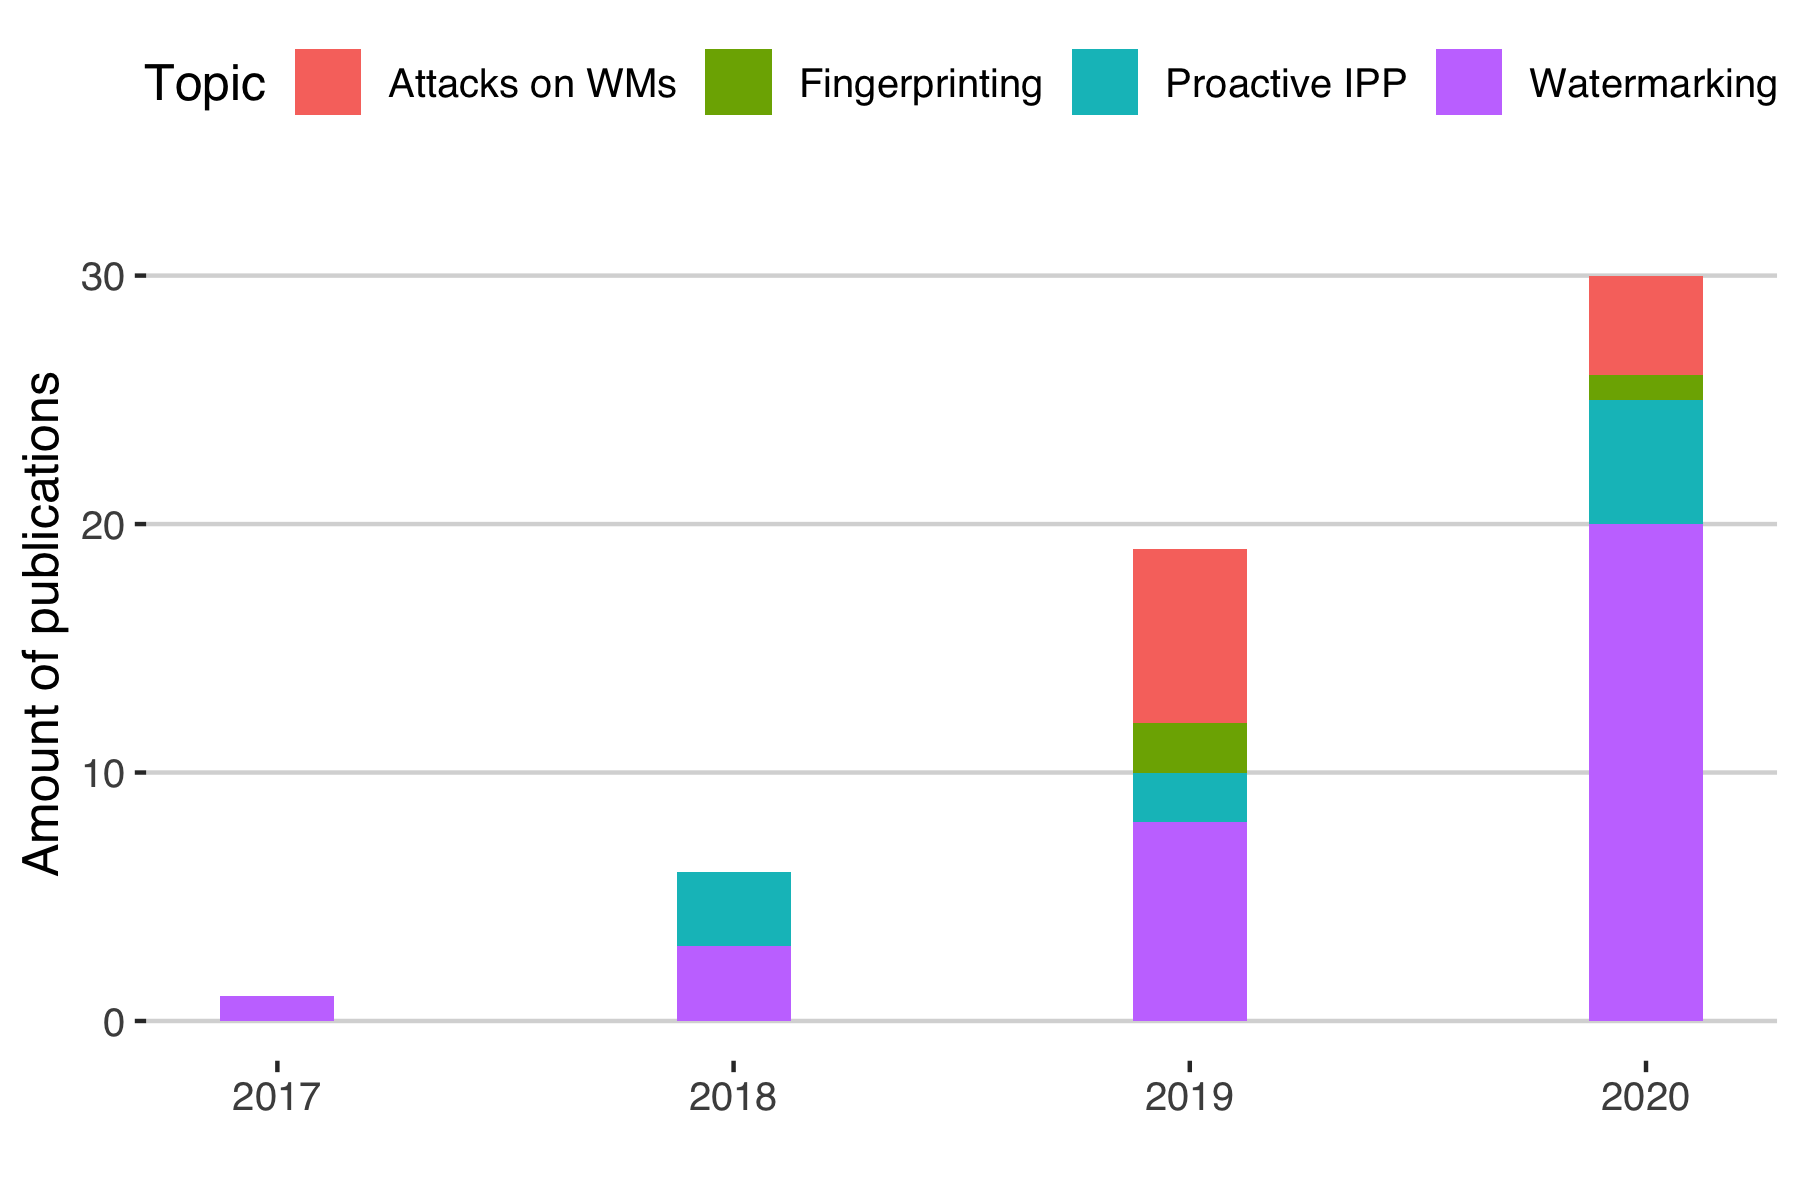
\includegraphics[width = \linewidth]{images/literature_years.png}
 \caption{Across the years for different topics}
 \label{fig:aufteilung-jahre}
 \end{subfigure}
 \caption{Literature distribution}
 \end{figure}

\cref{fig:aufteilung} shows the distribution of publications across the different topics in the various literature types. \textit{Attacks on WMs} include papers that propose attacks specifically crafted to disable a watermarking method or render it useless. \textit{Fingerprinting} and \textit{Watermarking} includes papers proposing a fingerprinting or watermarking method for ML models. \textit{Proactive IPP} includes papers on unrobust models and model access methods (cf. \cref{fig:overview}); these are not in the focus and are not discussed in more detail in this thesis. We can see that most papers were published regarding watermarking; however, there is also a significant number of papers on attacks published. Note, that some publications include both a novel attack to a scheme and a novel watermarking scheme, which is immune to this attack. Also, not all publications covering attacks are classified as such, as there is often a specific attack to a scheme, and a novel scheme immune to this attack, proposed in the same publication.

\cref{fig:aufteilung-jahre}, on the other hand, shows the distribution of publications across the publishing years. We see a rise in interest for this topic, with papers on attacks being mostly published in the last two years only.

\subsection{Inclusion/exclusion criteria} \label{appendix:method:criteria}

In order to provide reproducible documentation of the literature research, we defined the following inclusion and exclusion criteria to find the most relevant literature for the topic of IPP of ML models. Our inclusion criteria are:
\begin{itemize}
    \item Literature which proposes an IPP scheme for ML models
    \item Literature which proposes an attack on an IPP scheme for ML models
    \item Literature which evaluates or compares earlier schemes
\end{itemize}

Our exclusion criteria are:
\begin{itemize}
    \item (Near) Duplicates \footnote{If the titles are different but the content is very similar, we include all versions of the literature and note that. Later on, we will cite only the most complete version as suggested by Kitchenham et al. \cite{kitchenham_guidelines_2007}.}
    \item Literature which only \textit{uses} ML for multimedia watermarking, such as image watermarking
    \item Literature that only \textit{applies} previously published IP protection schemes, without a novel or large-scale evaluation
\end{itemize}

\section{Empirical evaluation}

As a first step we formulate research questions and define a study setting in \cref{ch:study_setting}, which includes benchmark architectures and datasets. We choose watermarking methods according to our defined selection criteria (cf. \cref{ch:study_setting}) and implement them in \cref{sec:implementation}. Afterwards, we analyse them based on experiments in \cref{sec:evaluation}. We synthesise our findings, answer the research questions and formulate selection guidelines in \cref{ch:conclusions}.

%1. research questions
%2. define study setting by choosing benchmark architectures and datasets
%3. choose wm methods
%4. implement wm methods
%5. run experiments
%6. synthesize finding -> answer research questions

%For the empirical evaluation of the chosen backdoor-based watermarking methods, we, first, define the study setting depending on the previously found key parameters. in order to find answers to our research questions. The research questions and the study setting are discussed in \cref{ch:study_setting}. Afterwards, we are going to implement the watermarking methods in a common framework, and evaluate and compare the methods regarding three main requirements for model watermarking in \cref{ch:empirical_comparison}.